\documentclass{article}

% if you need to pass options to natbib, use, e.g.:
% \PassOptionsToPackage{numbers, compress}{natbib}
% before loading nips_2016
%
% to avoid loading the natbib package, add option nonatbib:
% \usepackage[nonatbib]{nips_2016}

% \usepackage{nips_2016}

% to compile a camera-ready version, add the [final] option, e.g.:
\usepackage[final]{nips_2016}

\usepackage[utf8]{inputenc} % allow utf-8 input
\usepackage[T1]{fontenc}    % use 8-bit T1 fonts
\usepackage{hyperref}       % hyperlinks
\usepackage{url}            % simple URL typesetting
\usepackage{booktabs}       % professional-quality tables
\usepackage{amsfonts}       % blackboard math symbols
\usepackage{nicefrac}       % compact symbols for 1/2, etc.
\usepackage{microtype}      % microtypography
\usepackage{amssymb}
\usepackage{mathbbol}
\usepackage{graphicx}

\title{10-703 - Homework 2: Playing Atari With Deep Reinforcement Learning}

% The \author macro works with any number of authors. There are two
% commands used to separate the names and addresses of multiple
% authors: \And and \AND.
%
% Using \And between authors leaves it to LaTeX to determine where to
% break the lines. Using \AND forces a line break at that point. So,
% if LaTeX puts 3 of 4 authors names on the first line, and the last
% on the second line, try using \AND instead of \And before the third
% author name.

\author{
  Rogerio~Bonatti\ \\
  Robotics Institute\\
  Carnegie Mellon University\\
  Pittsburgh, PA 15213 \\
  \texttt{rbonatti@andrew.cmu.edu} \\
  %% examples of more authors
  \And
  Ratnesh~Madaan\ \\
  Robotics Institute\\
  Carnegie Mellon University\\
  Pittsburgh, PA 15213 \\
  \texttt{ratneshm@andrew.cmu.edu} \\
  %% \AND
  %% Coauthor \\
  %% Affiliation \\
  %% Address \\
  %% \texttt{email} \\
  %% \And
  %% Coauthor \\
  %% Affiliation \\
  %% Address \\
  %% \texttt{email} \\
  %% \And
  %% Coauthor \\
  %% Affiliation \\
  %% Address \\
  %% \texttt{email} \\
}

\begin{document}
% \nipsfinalcopy is no longer used

\maketitle

\begin{abstract}
  In this assignment we implemented Q-learning using deep learning function approximators for the Space Invaders game in the OpenAI Gym environment. We implemented the following variations of Q-learning: linear network without and with experience replay and target fixing, linear double Q-network with experience replay and target fixing, and dueling deep Q-learning. 
\end{abstract}

\section{[5pts] Show that update \ref{eq:updateQ} and update \ref{eq:updatew} are the same when the functions in $Q$ are of the form $Q_w(s,a) = w^T\phi(s,a)$, with $w \in \mathbb{R}^{|S||A|}$ and $\phi: S \times A \rightarrow \mathbb{R}^{|S||A|}$, where the feature function $\phi$ is of the form $\phi(s,a)_{s',a'} = \mathbb{1}[s'=s, a'=a]$}

Updates:

\begin{equation} \label{eq:updateQ}
  Q(s,a) := Q(s,a) + \alpha \left(r+\gamma \max_{a' \in A} Q(s',a') - Q(s,a)\right) 
\end{equation}

\begin{equation} \label{eq:updatew}
  w := w + \alpha \left(r+\gamma \max_{a' \in A} Q(s',a') - Q(s,a)\right) \nabla_w  Q_w(s,a)
\end{equation}

\textbf{Solution:}

We begin with Eq~\ref{eq:updatew}, substituting the derivative with respect to $w$, given that $Q(s,a)=w^T\phi(s,a)$:

\begin{equation} \label{eq:derivation_1}
  w := w + \alpha \left(r+\gamma \max_{a' \in A} Q(s',a') - Q(s,a)\right) \phi(s,a)
\end{equation}

Now we transpose both sides of the equation, and multiply both sides by $\phi(s,a)$:

\begin{equation} \label{eq:derivation_2}
  w^T\phi(s,a) := w^T\phi(s,a) + \alpha \left(r+\gamma \max_{a' \in A} Q(s',a') - Q(s,a)\right) \phi^T(s,a) \phi(s,a)
\end{equation}

Now we can again use the fact that $Q(s,a)=w^T\phi(s,a)$:

\begin{equation} \label{eq:derivation_3}
  Q(s,a) := Q(s,a) + \alpha \left(r+\gamma \max_{a' \in A} Q(s',a') - Q(s,a)\right) \phi^T(s,a) \phi(s,a)
\end{equation}

Lastly, since $\phi(s,a)_{s',a'} = \mathbb{1}[s'=s, a'=a]$, the norm of the dot product will equal to 1, resulting in:

\begin{equation} \label{eq:derivation_4}
  Q(s,a) := Q(s,a) + \alpha \left(r+\gamma \max_{a' \in A} Q(s',a') - Q(s,a)\right)
\end{equation}

And this we proved that Eq~\ref{eq:updatew} is the same as Eq~\ref{eq:updateQ}.

\section{[5pts] Implement a linear Q-network (no experience replay or target fixing). Use the experimental setup of \cite{mnih2013playing,mnih2015human} to the extent possible}

We implemented a linear Q-network, and to run the training process, one needs to run the command ``python dqn.py --modes ''.

We used the following hyper-parameters for this network:
\begin{itemize}
  \item Discount factor $\gamma=0.99$
  \item Learning rate $\alpha=0.0001$
  \item Exploration probability $\epsilon=0.05$, decreasing from $1$ to $0.05$ in a linear fashion during training process
  \item Number of iterations with environment: 5,000,000
  \item Number of frames to feed to the Q-network: 4
  \item Input image resizing: $84\times84$
  % \item Replay buffer size: 1,000,000
  % \item Target Q-network reset interval: 10,000
  % \item Batch size: 32
  \item Steps between evaluations of network: 10,000
  \item Steps for ``burn in'' (random actions in the beginning of training process): 50,000
  \item Maximum episode length: 100,000 steps (basically we chose to allow any game size)
\end{itemize}

We plotted the performance plots of this network in Figs~\ref{fig:q_q2}-\ref{fig:r_q2}.

\begin{figure}[ht] \label{fig:q_q2}
  \centering
  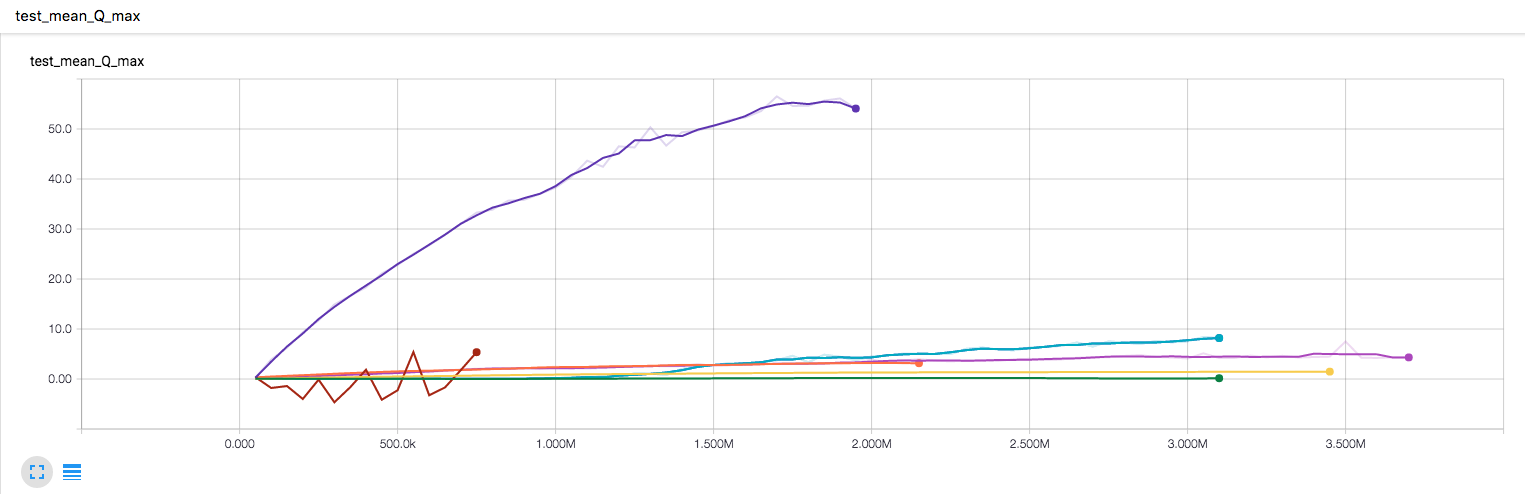
\includegraphics[width=1.0\textwidth]{images/q_linearWithoutStuff}
  \caption{Mean Q per step plot for the case of linear network without target fixing and without experience replay}
\end{figure}

\begin{figure}[ht] \label{fig:r_q2}
  \centering
  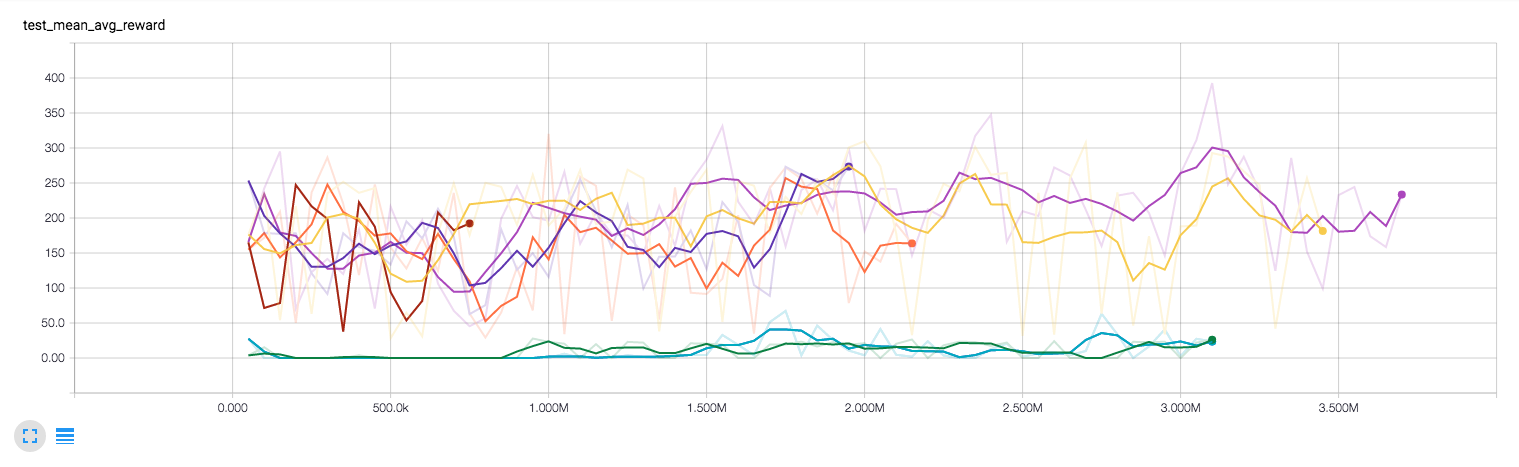
\includegraphics[width=1.0\textwidth]{images/r_linearWithoutStuff}
  \caption{Mean reward per episode plot for the case of linear network without target fixing and without experience replay}
\end{figure}

Using the \textit{Monitor} wrapper of the gym environment, we generated videos of the behavior of the agent across different stages of training:

\begin{itemize}
  \item 0/3 of training: \href{http://www.sharelatex.com}{Youtube video}
  \item 1/3 of training: \href{http://www.sharelatex.com}{Youtube video}
  \item 2/3 of training: \href{http://www.sharelatex.com}{Youtube video}
  \item 3/3 of training: \href{http://www.sharelatex.com}{Youtube video}
\end{itemize}

Here are also some comments about the behavior and training of this specific network:

\begin{itemize}
  \item Bla
  \item Bla
\end{itemize}


\section{[10pts] Implement a linear Q-network with experience replay and target fixing. Use the experimental setup of \cite{mnih2013playing,mnih2015human} to the extent possible}

We implemented a linear Q-network, and to run the training process, one needs to run the command ``python dqn.py --modes ''.

We used the following hyper-parameters for this network:
\begin{itemize}
  \item Discount factor $\gamma=0.99$
  \item Learning rate $\alpha=0.0001$
  \item Exploration probability $\epsilon=0.05$, decreasing from $1$ to $0.05$ in a linear fashion during training process
  \item Number of iterations with environment: 5,000,000
  \item Number of frames to feed to the Q-network: 4
  \item Input image resizing: $84\times84$
  \item Replay buffer size: 1,000,000
  \item Target Q-network reset interval: 10,000
  \item Batch size: 32
  \item Steps between evaluations of network: 10,000
  \item Steps for ``burn in'' (random actions in the beginning of training process): 50,000
  \item Maximum episode length: 100,000 steps (basically we chose to allow any game size)
\end{itemize}

We plotted the performance plots of this network in Figs~\ref{fig:q_q3}-\ref{fig:r_q3}.

% \begin{figure}[ht] \label{fig:q_q3}
%   \centering
%   \includegraphics[width=1.0\textwidth]{images/q_q3}
%   \caption{Mean Q per step plot for the case of linear network with target fixing and with experience replay}
% \end{figure}

% \begin{figure}[ht] \label{fig:r_q3}
%   \centering
%   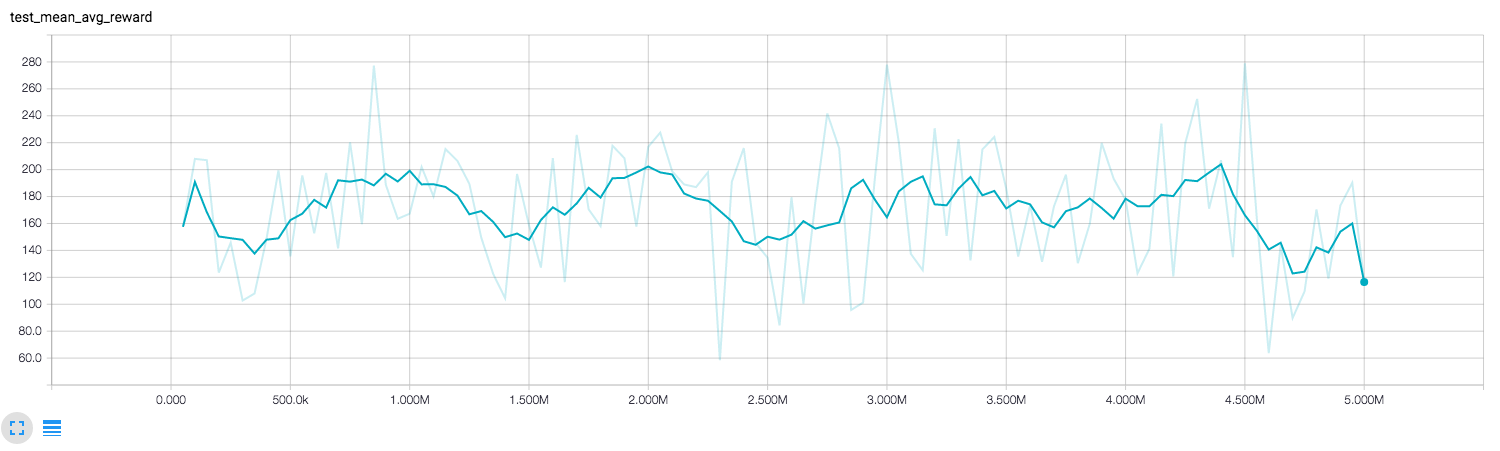
\includegraphics[width=1.0\textwidth]{images/r_q3}
%   \caption{Mean reward per episode plot for the case of linear network with target fixing and with experience replay}
% \end{figure}

Using the \textit{Monitor} wrapper of the gym environment, we generated videos of the behavior of the agent across different stages of training:

\begin{itemize}
  \item 0/3 of training: \href{http://www.sharelatex.com}{Youtube video}
  \item 1/3 of training: \href{http://www.sharelatex.com}{Youtube video}
  \item 2/3 of training: \href{http://www.sharelatex.com}{Youtube video}
  \item 3/3 of training: \href{http://www.sharelatex.com}{Youtube video}
\end{itemize}

Here are also some comments about the behavior and training of this specific network:

\begin{itemize}
  \item Bla
  \item Bla
\end{itemize}

\section{[5pts] Implement a linear double Q-network. Use the the experimental setup of \cite{mnih2013playing,mnih2015human} to the extent possible.}

We implemented a double linear Q-network, and to run the training process, one needs to run the command ``python dqn.py --modes ''.

We used the following hyper-parameters for this network:
\begin{itemize}
  \item Discount factor $\gamma=0.99$
  \item Learning rate $\alpha=0.0001$
  \item Exploration probability $\epsilon=0.05$, decreasing from $1$ to $0.05$ in a linear fashion during training process
  \item Number of iterations with environment: 5,000,000
  \item Number of frames to feed to the Q-network: 4
  \item Input image resizing: $84\times84$
  \item Replay buffer size: 1,000,000
  \item Target Q-network reset interval: 10,000
  \item Batch size: 32
  \item Steps between evaluations of network: 10,000
  \item Steps for ``burn in'' (random actions in the beginning of training process): 50,000
  \item Maximum episode length: 100,000 steps (basically we chose to allow any game size)
\end{itemize}

We plotted the performance plots of this network in Figs~\ref{fig:q_q4}-\ref{fig:r_q4}.

% \begin{figure}[ht] \label{fig:q_q4}
%   \centering
%   \includegraphics[width=1.0\textwidth]{images/q_q4}
%   \caption{Mean Q per step plot for the case of double linear network with target fixing and with experience replay}
% \end{figure}

% \begin{figure}[ht] \label{fig:r_q4}
%   \centering
%   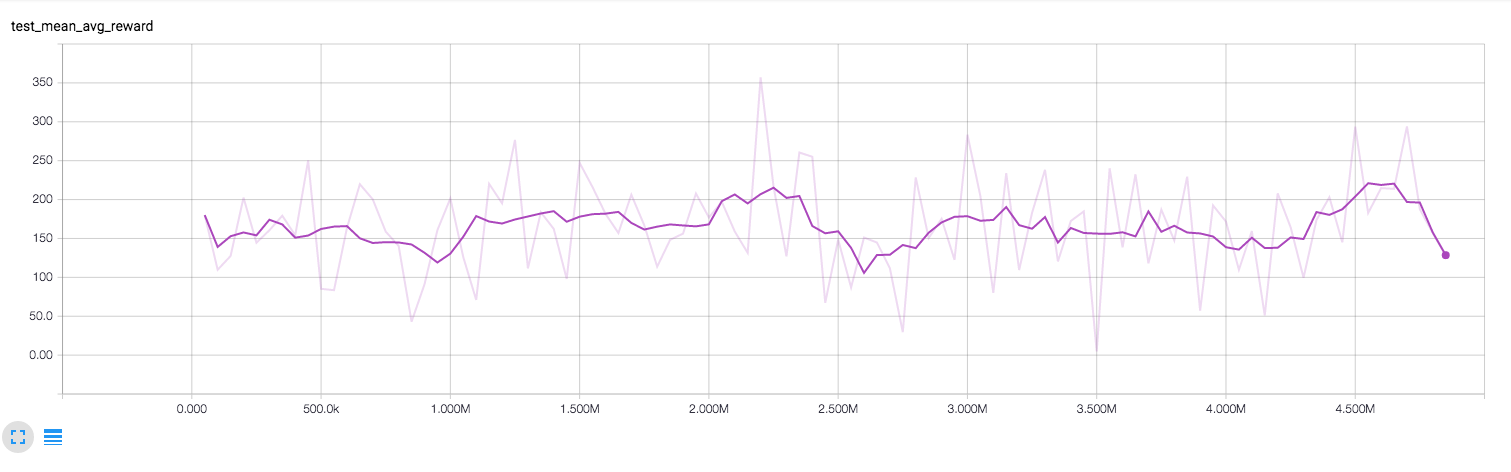
\includegraphics[width=1.0\textwidth]{images/r_q4}
%   \caption{Mean reward per episode plot for the case of double linear network with target fixing and with experience replay}
% \end{figure}

Using the \textit{Monitor} wrapper of the gym environment, we generated videos of the behavior of the agent across different stages of training:

\begin{itemize}
  \item 0/3 of training: \href{http://www.sharelatex.com}{Youtube video}
  \item 1/3 of training: \href{http://www.sharelatex.com}{Youtube video}
  \item 2/3 of training: \href{http://www.sharelatex.com}{Youtube video}
  \item 3/3 of training: \href{http://www.sharelatex.com}{Youtube video}
\end{itemize}

Here are also some comments about the behavior and training of this specific network:

\begin{itemize}
  \item Bla
  \item Bla
\end{itemize}

\section{[35pts] Implement the deep Q-network as described in \cite{mnih2013playing,mnih2015human}}

We implemented a deep Q-network. We tested the performance of this network with different games, and to run them, one can use the following commands:
\begin{itemize}
  \item Space invaders: ``python dqn.py --modes ''
  \item Enduro: ``python dqn.py --modes ''
  \item Breakout: ``python dqn.py --modes ''
\end{itemize}

We used the following hyper-parameters for this network:
\begin{itemize}
  \item Discount factor $\gamma=0.99$
  \item Learning rate $\alpha=0.0001$
  \item Exploration probability $\epsilon=0.05$, decreasing from $1$ to $0.05$ in a linear fashion during training process
  \item Number of iterations with environment: 5,000,000
  \item Number of frames to feed to the Q-network: 4
  \item Input image resizing: $84\times84$
  \item Replay buffer size: 1,000,000
  \item Target Q-network reset interval: 10,000
  \item Batch size: 32
  \item Steps between evaluations of network: 10,000
  \item Steps for ``burn in'' (random actions in the beginning of training process): 50,000
  \item Maximum episode length: 100,000 steps (basically we chose to allow any game size)
\end{itemize}

We plotted the performance plots of this network in for different games in Figs~\ref{fig:q_q4}-\ref{fig:r_q4}.

% \begin{figure}[ht] \label{fig:q_q5_space}
%   \centering
%   \includegraphics[width=1.0\textwidth]{images/q_q5_space}
%   \caption{Mean Q per step plot for Space Invaders for the case of deep Q network with target fixing and with experience replay}
% \end{figure}

% \begin{figure}[ht] \label{fig:r_q5_space}
%   \centering
%   \includegraphics[width=1.0\textwidth]{images/r_q5_space}
%   \caption{Mean reward per episode plot for Space Invaders for the case of deep Q network with target fixing and with experience replay}
% \end{figure}

% \begin{figure}[ht] \label{fig:q_q5_enduro}
%   \centering
%   \includegraphics[width=1.0\textwidth]{images/q_q5_enduro}
%   \caption{Mean Q per step plot for Enduro for the case of deep Q network with target fixing and with experience replay}
% \end{figure}

% \begin{figure}[ht] \label{fig:r_q5_enduro}
%   \centering
%   \includegraphics[width=1.0\textwidth]{images/r_q5_enduro}
%   \caption{Mean reward per episode plot for Enduro for the case of deep Q network with target fixing and with experience replay}
% \end{figure}

% \begin{figure}[ht] \label{fig:q_q5_breakout}
%   \centering
%   \includegraphics[width=1.0\textwidth]{images/q_q5_breakout}
%   \caption{Mean Q per step plot for Breakout for the case of deep Q network with target fixing and with experience replay}
% \end{figure}

% \begin{figure}[ht] \label{fig:r_q5_breakout}
%   \centering
%   \includegraphics[width=1.0\textwidth]{images/r_q5_breakout}
%   \caption{Mean reward per episode plot for Breakout for the case of deep Q network with target fixing and with experience replay}
% \end{figure}

Using the \textit{Monitor} wrapper of the gym environment, we generated videos of the behavior of the agent across different stages of training, for the 3 games considered:

For Space invaders:
\begin{itemize}
  \item 0/3 of training: \href{http://www.sharelatex.com}{Youtube video}
  \item 1/3 of training: \href{http://www.sharelatex.com}{Youtube video}
  \item 2/3 of training: \href{http://www.sharelatex.com}{Youtube video}
  \item 3/3 of training: \href{http://www.sharelatex.com}{Youtube video}
\end{itemize}

For Enduro:
\begin{itemize}
  \item 0/3 of training: \href{http://www.sharelatex.com}{Youtube video}
  \item 1/3 of training: \href{http://www.sharelatex.com}{Youtube video}
  \item 2/3 of training: \href{http://www.sharelatex.com}{Youtube video}
  \item 3/3 of training: \href{http://www.sharelatex.com}{Youtube video}
\end{itemize}

For Breakout:
\begin{itemize}
  \item 0/3 of training: \href{http://www.sharelatex.com}{Youtube video}
  \item 1/3 of training: \href{http://www.sharelatex.com}{Youtube video}
  \item 2/3 of training: \href{http://www.sharelatex.com}{Youtube video}
  \item 3/3 of training: \href{http://www.sharelatex.com}{Youtube video}
\end{itemize}

Here are also some comments about the behavior and training of this specific network:

\begin{itemize}
  \item Bla
  \item Bla
\end{itemize}

\section{[20pts] Implement the double deep Q-network as described in \cite{van2016deep}}

We implemented a double deep Q-network, and to run the training process, one needs to run the command ``python dqn.py --modes ''.

We used the following hyper-parameters for this network:
\begin{itemize}
  \item Discount factor $\gamma=0.99$
  \item Learning rate $\alpha=0.0001$
  \item Exploration probability $\epsilon=0.05$, decreasing from $1$ to $0.05$ in a linear fashion during training process
  \item Number of iterations with environment: 5,000,000
  \item Number of frames to feed to the Q-network: 4
  \item Input image resizing: $84\times84$
  \item Replay buffer size: 1,000,000
  \item Target Q-network reset interval: 10,000
  \item Batch size: 32
  \item Steps between evaluations of network: 10,000
  \item Steps for ``burn in'' (random actions in the beginning of training process): 50,000
  \item Maximum episode length: 100,000 steps (basically we chose to allow any game size)
\end{itemize}

We plotted the performance plots of this network for Space Invaders in Figs~\ref{fig:q_q6}-\ref{fig:r_q6}.

% \begin{figure}[ht] \label{fig:q_q6}
%   \centering
%   \includegraphics[width=1.0\textwidth]{images/q_q6}
%   \caption{Mean Q per step plot for the case of double linear network with target fixing and with experience replay}
% \end{figure}

% \begin{figure}[ht] \label{fig:r_q6}
%   \centering
%   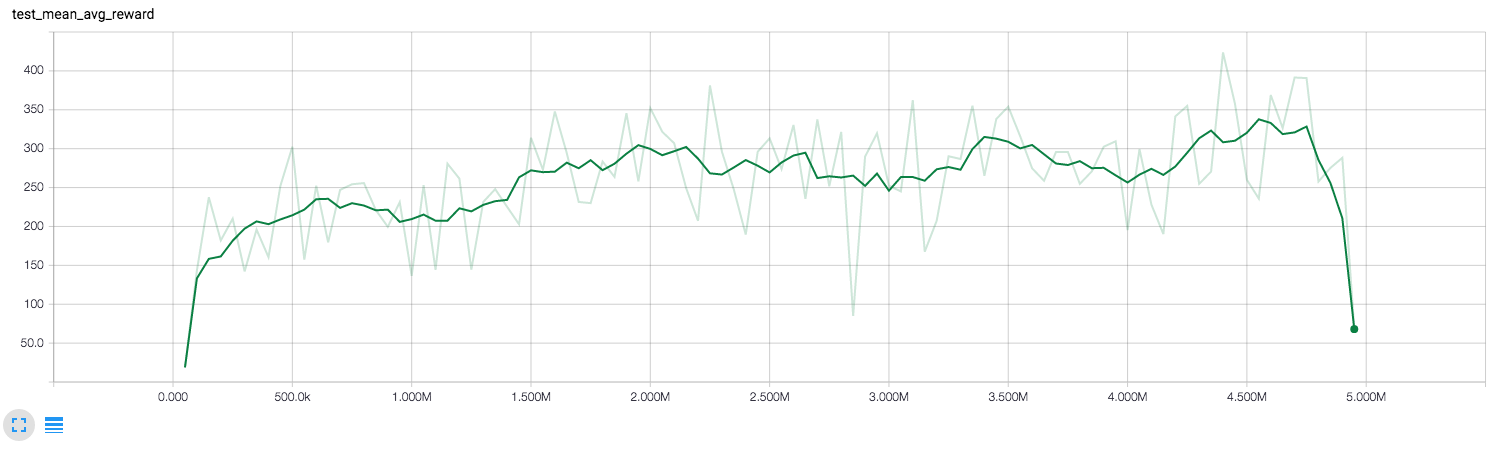
\includegraphics[width=1.0\textwidth]{images/r_q6}
%   \caption{Mean reward per episode plot for the case of double linear network with target fixing and with experience replay}
% \end{figure}

Using the \textit{Monitor} wrapper of the gym environment, we generated videos of the behavior of the agent across different stages of training:

\begin{itemize}
  \item 0/3 of training: \href{http://www.sharelatex.com}{Youtube video}
  \item 1/3 of training: \href{http://www.sharelatex.com}{Youtube video}
  \item 2/3 of training: \href{http://www.sharelatex.com}{Youtube video}
  \item 3/3 of training: \href{http://www.sharelatex.com}{Youtube video}
\end{itemize}

Here are also some comments about the behavior and training of this specific network:

\begin{itemize}
  \item Bla
  \item Bla
\end{itemize}

\section{[20pts] Implement the dueling deep Q-network as described in \cite{wang2015dueling}}

We implemented a dueling deep Q-network, and to run the training process, one needs to run the command ``python dqn.py --modes ''.

We used the following hyper-parameters for this network:
\begin{itemize}
  \item Discount factor $\gamma=0.99$
  \item Learning rate $\alpha=0.0001$
  \item Exploration probability $\epsilon=0.05$, decreasing from $1$ to $0.05$ in a linear fashion during training process
  \item Number of iterations with environment: 5,000,000
  \item Number of frames to feed to the Q-network: 4
  \item Input image resizing: $84\times84$
  \item Replay buffer size: 1,000,000
  \item Target Q-network reset interval: 10,000
  \item Batch size: 32
  \item Steps between evaluations of network: 10,000
  \item Steps for ``burn in'' (random actions in the beginning of training process): 50,000
  \item Maximum episode length: 100,000 steps (basically we chose to allow any game size)
\end{itemize}

We plotted the performance plots of this network in Figs~\ref{fig:q_q7}-\ref{fig:r_q7}.

% \begin{figure}[ht] \label{fig:q_q7}
%   \centering
%   \includegraphics[width=1.0\textwidth]{images/q_q7}
%   \caption{Mean Q per step plot for the case of double linear network with target fixing and with experience replay}
% \end{figure}

% \begin{figure}[ht] \label{fig:r_q7}
%   \centering
%   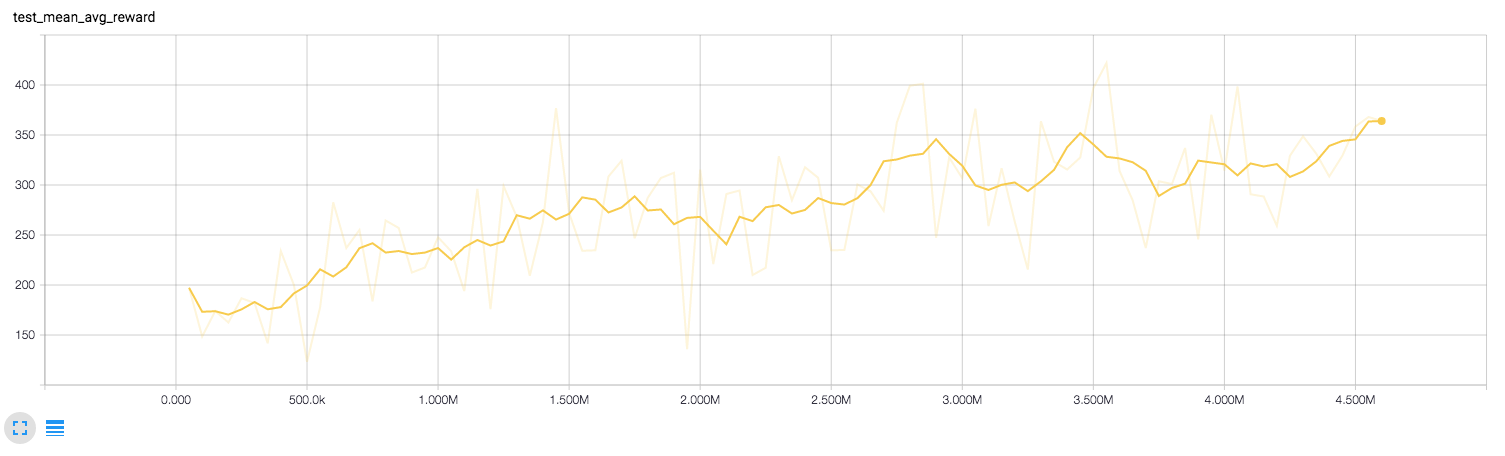
\includegraphics[width=1.0\textwidth]{images/r_q7}
%   \caption{Mean reward per episode plot for the case of double linear network with target fixing and with experience replay}
% \end{figure}

Using the \textit{Monitor} wrapper of the gym environment, we generated videos of the behavior of the agent across different stages of training:

\begin{itemize}
  \item 0/3 of training: \href{http://www.sharelatex.com}{Youtube video}
  \item 1/3 of training: \href{http://www.sharelatex.com}{Youtube video}
  \item 2/3 of training: \href{http://www.sharelatex.com}{Youtube video}
  \item 3/3 of training: \href{http://www.sharelatex.com}{Youtube video}
\end{itemize}

Here are also some comments about the behavior and training of this specific network:

\begin{itemize}
  \item Bla
  \item Bla
\end{itemize}

\section{Table comparing rewards for each fully trained model} % (fold)
\label{sec:table_comparing_rewards_for_each_fully_trained_model}
We constructed a table comparing the average total reward found in 100 episodes for each fully trained model we implemented:

\begin{table}[h]
  \caption{Avg reward per episode for 100 episodes in implemented networks}
  \label{sample-table}
  \centering
  \begin{tabular}{lll}
    \toprule

    Model     & Game     & Avg Reward 100 episodes \\
    \midrule
    Linear, no target fix, no exp replay & Space Invaders  & $50\pm5$     \\
    Linear, with target fix, with exp replay & Space Invaders  & $50\pm5$     \\
    Double Linear & Space Invaders  & $50\pm5$     \\
    Deep Q & Space Invaders  & $50\pm5$     \\
    Deep Q & Enduro  & $50\pm5$     \\
    Deep Q & Breakout  & $50\pm5$     \\
    Double Deep Q & Space Invaders  & $50\pm5$     \\
    Dueling Deep Q & Space Invaders  & $50\pm5$     \\
    \bottomrule
  \end{tabular}
\end{table}

Here are some comments about the results in the table:
\begin{itemize}
  \item Bla
  \item Bla
\end{itemize}
% section table_comparing_rewards_for_each_fully_trained_model (end)


\small
\medskip
\bibliographystyle{plain}
\bibliography{bibliography}

% References follow the acknowledgments. Use unnumbered first-level
% heading for the references. Any choice of citation style is acceptable
% as long as you are consistent. It is permissible to reduce the font
% size to \verb+small+ (9 point) when listing the references. {\bf
%   Remember that you can use a ninth page as long as it contains
%   \emph{only} cited references.}




% [1] Alexander, J.A.\ \& Mozer, M.C.\ (1995) Template-based algorithms
% for connectionist rule extraction. In G.\ Tesauro, D.S.\ Touretzky and
% T.K.\ Leen (eds.), {\it Advances in Neural Information Processing
%   Systems 7}, pp.\ 609--616. Cambridge, MA: MIT Press.

% [2] Bower, J.M.\ \& Beeman, D.\ (1995) {\it The Book of GENESIS:
%   Exploring Realistic Neural Models with the GEneral NEural SImulation
%   System.}  New York: TELOS/Springer--Verlag.

% [3] Hasselmo, M.E., Schnell, E.\ \& Barkai, E.\ (1995) Dynamics of
% learning and recall at excitatory recurrent synapses and cholinergic
% modulation in rat hippocampal region CA3. {\it Journal of
%   Neuroscience} {\bf 15}(7):5249-5262.

\end{document}
